%% initialising preamble
\documentclass[12pt, xcolor=table]{beamer}  %, handout

%% choosing theme and colortheme
\usetheme[secheader]{Boadilla}
\usecolortheme{dolphin}

%% loading packages
\usepackage{animate}	%% Animate graphs
\usepackage{amsmath}    %% Better math support
\usepackage{amssymb}
\usepackage{bm}			%% Bold math 
\usepackage{booktabs}	%% Better tables
\usepackage{hyperref}	%% Referencing
\usepackage{ragged2e}
\usepackage{setspace}	%% Space between bullets of list
%\usepackage[table]{xcolor}		%% For rowcolors in tables

%% setting beamer templates
\setbeamertemplate{navigation symbols}{}
\setbeamertemplate{section in toc}{\hspace*{1em}\inserttocsection}
\setbeamertemplate{subsection in toc}{\hspace*{2em}\textsl \inserttocsubsection \par}%
\setbeamertemplate{itemize items}[triangle]
%\setbeamertemplate{frametitle}[default][center]

%% some colors
\definecolor{White}{RGB}{255,255,255}
\definecolor{Red}{rgb}{0.9,0.15,0}
\definecolor{Blue}{RGB}{55,126,184}
\definecolor{Green}{RGB}{77,175,74}
\definecolor{grey}{RGB}{220,220,220}
\definecolor{myInfant}{RGB}{186,85,211}
\definecolor{mySenescent}{RGB}{255,140,0}
\definecolor{myAccident}{RGB}{0,128,255}

%% title information
\title[PhD defence]{
$\,$\\ \bigskip \Large{\textsc{New Approaches in Mortality \\ Modelling and Forecasting}}\\$\,$\\}
\subtitle{\large{\textsl{Assessment of PhD dissertation}}}

%% author information
%\author[Ugofilippo Basellini]{\large \textsl{Assessment of PhD dissertation} \\ $\,$ \\ Ugofilippo Basellini
%}

\author[Ugofilippo Basellini]
{%
	\vspace{-0.75cm}
	\texorpdfstring{
		\bigskip \large{Ugofilippo Basellini} \\
		\bigskip
		\medskip
		\includegraphics[scale=1.1]{Figures/Ch0/logo-banner.png} $\qquad$ \includegraphics[scale=0.235]{Figures/Ch0/ined_Hc_couleur.jpg} 
		\bigskip
		\medskip
		\begin{columns}%[onlytextwidth]
			\column{0.97\linewidth}
			\scriptsize{\textbf{Assessment Committee}}:\\
			Assoc.~Prof.~Fanny Janssen \hfill{University of Southern Denmark}\\
			Dr.~Iain D.~Currie \hfill{Department of Public Health}\\
			Prof.~Mauro Laudicella (chairman) \hfill{Odense, 24$^{\mathrm{th}}$ February 2020} \\   
		\end{columns}
	}
	{}
}

%% date information
%\date[]{\small \emph{University of Southern Denmark \\ Department of Public Health \\ 24$^{th}$ February 2020}}
\date{}

%% customize table of content
%\AtBeginSection[]{
%	\begin{frame}
%	\frametitle{Outline}
%	\tableofcontents[currentsection]
%\end{frame}
%}
%
%\AtBeginSubsection[]{
%	\begin{frame}
%	\frametitle{Outline}
%	\tableofcontents[currentsubsection]
%\end{frame}
%}



%%%%%%%%%%%%%%%%%%%%%%%%%%%%%%%%%%%%%%%%%%%%%%%%%%%%%%%%%%%%%%%%%%%%%
%%%%%%%%%%%%%%%%%%%%%%%%%%%%%%%%%%%%%%%%%%%%%%%%%%%%%%%%%%%%%%%%%%%%%

%% start of main document
\begin{document}

%% title page
\begin{frame}[plain]
	\titlepage
\end{frame}

\begin{frame}[plain]\frametitle{Thesis overview}
	\textbf{Five chapters}: 
	\begin{itemize}
	\scriptsize	
	\item Basellini, Canudas-Romo and Lenart (2019). Location--Scale Models in Demography: A Useful Re-parameterization of Mortality Models. {\it European Journal of Population}, {\bf 35}, 645\,--\,673.
	
	\item Basellini and Camarda (2019). Modelling and forecasting adult age-at-death distributions. {\it Population Studies}, {\bf 73}(1), 119\,--\,138.
	
	\item Basellini and Camarda (2020). A Three-component Approach to Model and Forecast Age-at-death Distributions. In Mazzuco, S., and Keilman, N. (eds.), {\it Developments in Demographic
	Forecasting}, Springer. Forthcoming.
	
	\item Basellini, Kj{\ae}rgaard and Camarda (2020). An age-at-death distribution approach \\ to forecast cohort mortality. {\it Insurance: Mathematics and Economics}, {\bf 91}, 129\,--\,143.	
	
	\item Camarda and Basellini. Smoothing, decomposing and forecasting mortality rates. Manuscript under review.	
	\end{itemize}
\bigskip 
	\textbf{Main goal of PhD thesis}: 
	\begin{itemize}
	\item introduce innovative methods to provide novel insights into the analysis and forecasting of human mortality	
	\end{itemize}
\end{frame}



%%%%%%%%%%%%%%%%%%%%%%%%%%%%%%%%%%%%%%%%%%%%%%%%%%%%%%%%%%%%%%%%%%%%%
%%%%%%%%% INTRODUCTION %%%%%%%%%%%%%%%%%%%%%%%%%%%%%%%%%%%%%%%%%%%%%%
%%%%%%%%%%%%%%%%%%%%%%%%%%%%%%%%%%%%%%%%%%%%%%%%%%%%%%%%%%%%%%%%%%%%%
%\section{Introduction}
%
%%% New frame
%\begin{frame}\frametitle{Motivation}
%
%\textbf{Background}:
%\begin{itemize}
%\setlength\itemsep{1.1em}
%\item mortality modelling and forecasting well established in demographic and actuarial sciences \pause
%\item current demographic challenges have stimulated renewed and increasing attention to this area of research \pause
%\end{itemize}
%\bigskip
%\medskip
%\textbf{Goal of PhD thesis}: 
%\begin{itemize}
%\item introduce innovative methods to provide novel insights into the analysis and forecasting of human mortality
%\end{itemize}
%
%\end{frame}

%% SPECIFIC GOALS
%\begin{frame}\frametitle{Specific goals of PhD thesis}
%\begin{itemize}
%\setlength\itemsep{1em}
%\item {\usebeamercolor[fg]{structure}Aim 1}: reconcile the most employed parametric models of mortality within a single overarching family \pause
%\item {\usebeamercolor[fg]{structure}Aim 2}: develop a new paradigm in mortality forecasting based on age-at-death distributions \pause
%\item {\usebeamercolor[fg]{structure}Aim 3}: investigate the rather unexplored area of cohort mortality forecasting \pause
%\item {\usebeamercolor[fg]{structure}Aim 4}: introduce the decomposition of the mortality age-pattern in mortality forecasts
%\end{itemize}
%\pause  
%\medskip
%\begin{center}
%$\Rightarrow$ 5 studies devised to address these goals
%\end{center}
%\end{frame}


%% APPLICATIONS
%\begin{frame}\frametitle{Focus of this presentation}
%\begin{itemize}
%	\setlength\itemsep{1.5em}
%	\item overview of the methodologies developed in the five studies \pause
%	\item application to Danish and Swedish female mortality data obtained from the Human Mortality Database (2020)
%	\begin{itemize}
%		\item period: years 1960--2016, all ages or adult ages (30--110+)
%		\item cohort: birth cohorts 1835--1970, ages 40--110+
%	\end{itemize}
%	 \pause
%	 \item forecasting comparisons with the most well-established methodology
%	 	\begin{itemize}
%	 	\item period: Lee and Carter (1992)
%	 	\item cohort: Currie et al.~(2004)
%	 \end{itemize}
%\end{itemize}
%\end{frame}

%%%%%%%%%%%%%%%%%%%%%%%%%%%%%%%%%%%%%%%%%%%%%%%%%%%%%%%%%%%%%%%%%%%%%
%%%%%%%%% CHAPTER 1 %%%%%%%%%%%%%%%%%%%%%%%%%%%%%%%%%%%%%%%%%%%%%%
%%%%%%%%%%%%%%%%%%%%%%%%%%%%%%%%%%%%%%%%%%%%%%%%%%%%%%%%%%%%%%%%%%%%%
\section{Chapter 1}
\subsection{Location--scale models in demography}

\begin{frame}[plain]\frametitle{Thesis overview}
	\textbf{Five chapters}: 
	\begin{itemize}
		\scriptsize	
		\item Basellini, Canudas-Romo and Lenart (2019). Location--Scale Models in Demography: A Useful Re-parameterization of Mortality Models. {\it European Journal of Population}, {\bf 35}, 645\,--\,673.
		
		\item {\pgfsetfillopacity{0.2} Basellini and Camarda (2019). Modelling and forecasting adult age-at-death distributions. {\it Population Studies}, {\bf 73}(1), 119\,--\,138.
		
		\item Basellini and Camarda (2020). A Three-component Approach to Model and Forecast Age-at-death Distributions. In Mazzuco, S., and Keilman, N. (eds.), {\it Developments in Demographic Forecasting}, Springer. Forthcoming.
		
		\item Basellini, Kj{\ae}rgaard and Camarda (2020). An age-at-death distribution approach \\ to forecast cohort mortality. {\it Insurance: Mathematics and Economics}, {\bf 91}, 129\,--\,143.	
		
		\item Camarda and Basellini. Smoothing, decomposing and forecasting mortality rates. Manuscript under review. }	
	\end{itemize}
	\bigskip
	{\pgfsetfillopacity{1} 
	\textbf{Main goal of PhD thesis}: 
	\begin{itemize}
		\item introduce innovative methods to provide novel insights into the analysis and forecasting of human mortality	
	\end{itemize}
}
\end{frame}


%%%%%%%% Motivation LS PAPER
\begin{frame} %\frametitle{Introduction}
\textbf{Background:}
\begin{itemize}
\setlength\itemsep{0.5em}
\item several parametric models proposed to describe the age-pattern of human mortality $\,$ % \hyperlink{ParamModels}{\beamerbutton{some examples}} 
%\hypertarget{ParamModelsBACK}{}
\item few efforts to reunite most models within a single framework \scriptsize{(some exceptions: Currie 2016; Forfar et al.~1988)}
\end{itemize}
\bigskip \pause
\textbf{Objective:} reconcile the most common parametric models of mortality within a single overarching family \\
\bigskip \pause
\textbf{Contribution:} propose the location--scale (LS) family as unifying framework in mortality modelling
\begin{itemize}
\setlength\itemsep{0.5em}
\item several models belong to the family %$\,$ \hyperlink{LSModels}{\beamerbutton{list of models}} 
%\hypertarget{LSModelsBACK}{}
\item LS parameters simple and clear demographic interpretation: mortality shifting and compression
%\item desirable properties and statistical advantages % $\,$ \hyperlink{LSAdvantages}{\beamerbutton{LS advantages}}
%\hypertarget{LSAdvantagesBACK}{}
\end{itemize}

\end{frame}

%%%% LS MODEL: SHIFTING
\begin{frame}\frametitle{LS family}
	\begin{center}
		\vspace{0.15cm}
		\normalsize {\color{white}location (u): \textbf{shifting} mortality dynamic} \\
		\animategraphics[autoplay,palindrome,scale=0.45]{4}{Figures/Ch1/F2_anim_location}{0}{0}
	\end{center}
	
\end{frame}

%%%% LS MODEL: SHIFTING
\begin{frame}[noframenumbering]\frametitle{LS family}
	\begin{center}
		\vspace{0.15cm}
		\normalsize {\color{red}location (u)}: \textbf{shifting} mortality dynamic \\
		\animategraphics[autoplay,palindrome,scale=0.45]{4}{Figures/Ch1/F2_anim_location}{1}{1}
	\end{center}
	
\end{frame}

%%%% LS MODEL: SHIFTING
\begin{frame}[noframenumbering]\frametitle{LS family}
	\begin{center}
		\vspace{0.15cm}
		\normalsize {\color{red}location (u)}: \textbf{shifting} mortality dynamic \\
		\animategraphics[autoplay,palindrome,scale=0.45]{4}{Figures/Ch1/F2_anim_location}{1}{36}
	\end{center}
	
\end{frame}

%%%% LS MODEL: COMPRESSION
\begin{frame}\frametitle{LS family}
	\begin{center}
		\vspace{0.15cm}
		\normalsize {\color{blue}scale (c)}: \textbf{compression} mortality dynamic \\
		\animategraphics[autoplay,palindrome,scale=0.45]{4}{Figures/Ch1/F2_anim_scale}{0}{0}
	\end{center}
	
\end{frame}

%%%% LS MODEL: COMPRESSION
\begin{frame}[noframenumbering]\frametitle{LS family}
	\begin{center}
		\vspace{0.15cm}
		\normalsize {\color{blue}scale (c)}: \textbf{compression} mortality dynamic \\
		\animategraphics[autoplay,palindrome,scale=0.45]{4}{Figures/Ch1/F2_anim_scale}{0}{35}
	\end{center}
	
\end{frame}

%%%%%%%%% ADVANTAGES LS family
%\begin{frame}\frametitle{Results: LS estimates}
%\vspace{-0.25cm}
%\begin{center}
%\includegraphics[scale=0.45]{Figures/Ch1/F3_a}
%\end{center}
%\vspace{-0.3cm}
%\tiny{$\quad\quad\quad\quad$ Estimated LS parameters of the Minimal Generalized Extreme--Value model.\\ $\quad\quad\quad\quad$ Danish females, ages 30--110+, years 1960--2016. \\ \emph{$\quad\quad\quad\quad$ Source: HMD (2020)}} \\
%\hfill{\hyperlink{LSOtherModels}{\beamerbutton{other models}}}\\
%\hypertarget{LSOtherModelsBACK}{}
%
%\end{frame}

%%%%%%%% ADVANTAGES LS family
\begin{frame}\frametitle{Application: mortality shifting and compression}
\vspace{-0.25cm}
\begin{center}
\includegraphics[scale=0.45]{Figures/Ch1/F3_b}
\end{center}
\vspace{-0.3cm}
\tiny{$\quad\quad\quad\quad$ Estimated LS parameters of the Minimal Generalized Extreme--Value model (lowest BIC).\\ $\quad\quad\quad\quad$ Swedish and Danish females, ages 30--110+, years 1960--2016. \\ \emph{$\quad\quad\quad\quad$ Source: HMD (2020)}} %\\
%\hfill{\hyperlink{LSOtherModels}{\beamerbutton{different models}}}
%\hypertarget{LSOtherModelsBACK}{}

\end{frame}

%%%%%%%%%%%%%%%%%%%%%%%%%%%%%%%%%%%%%%%%%%%%%%%%%%%%%%%%%%%%%%%%%%%%%
%%%%%%%%% CHAPTER 2 %%%%%%%%%%%%%%%%%%%%%%%%%%%%%%%%%%%%%%%%%%%%%%
%%%%%%%%%%%%%%%%%%%%%%%%%%%%%%%%%%%%%%%%%%%%%%%%%%%%%%%%%%%%%%%%%%%%%
\section{Chapter 2}
\subsection{The STAD model}
\begin{frame}[plain]\frametitle{Thesis overview}
	\textbf{Five chapters}: 
	\begin{itemize}
		\scriptsize	
		\item {\pgfsetfillopacity{0.2} Basellini, Canudas-Romo and Lenart (2019). Location--Scale Models in Demography: A Useful Re-parameterization of Mortality Models. {\it European Journal of Population}, {\bf 35}, 645\,--\,673. }	
		
		\item  {\pgfsetfillopacity{1} Basellini and Camarda (2019). Modelling and forecasting adult age-at-death distributions. {\it Population Studies}, {\bf 73}(1), 119\,--\,138. }
			
		\item {\pgfsetfillopacity{0.2} Basellini and Camarda (2020). A Three-component Approach to Model and Forecast Age-at-death Distributions. In Mazzuco, S., and Keilman, N. (eds.), {\it Developments in Demographic Forecasting}, Springer. Forthcoming.
			
		\item Basellini, Kj{\ae}rgaard and Camarda (2020). An age-at-death distribution approach \\ to forecast cohort mortality. {\it Insurance: Mathematics and Economics}, {\bf 91}, 129\,--\,143.	
			
		\item Camarda and Basellini. Smoothing, decomposing and forecasting mortality rates. Manuscript under review. }	
	\end{itemize}
	\bigskip
	{\pgfsetfillopacity{1} 
		\textbf{Main goal of PhD thesis}: 
		\begin{itemize}
			\item introduce innovative methods to provide novel insights into the analysis and forecasting of human mortality	
		\end{itemize}
	}
\end{frame}


%%%%%%%% Motivation STAD PAPER
\begin{frame} %\frametitle{Introduction}
	\textbf{Background:}
	\begin{itemize}
		\setlength\itemsep{0.5em}
		\item mortality modeling and forecasting are generally based on mortality rates 
		\item age-at-death distributions are very informative, yet neglected for modeling and forecasting mortality
	\end{itemize}
	\bigskip \pause
	\textbf{Objective:} model and forecast adult mortality by studying changes in age-at-death distributions 
	\\ \bigskip \pause
	\textbf{Contribution:} propose the Segmented Transformation Age-at-Death Distributions (STAD) model to analyze and forecast adult mortality
	\begin{itemize}
		\setlength\itemsep{0.5em}
		\item parsimonious and efficient model 
		\item mortality forecasts more accurate and optimistic than the Lee-Carter model and its variants
	\end{itemize}
	
\end{frame}

%%%% MOTIVATION
%% MX developments
\begin{frame}\frametitle{Motivation}
\vspace{-0.2cm}
\begin{center}
\animategraphics[autoplay,scale=0.46]{5}{Figures/Ch2/F1_anim_LMX}{0}{28}
\end{center}
\vspace{-0.3cm}
\tiny{$\quad\quad\quad\quad$ Mortality rates (log scale). \\ $\quad\quad\quad\quad$ Swedish and Danish females, ages 30--110+, years 1960--2016. \\ \emph{$\quad\quad\quad\quad$ Source: HMD (2020)}}
\end{frame}

%%%% MOTIVATION
%% FX developments
\begin{frame}\frametitle{Motivation}
\vspace{-0.2cm}
\begin{center}
\animategraphics[autoplay,scale=0.46]{5}{Figures/Ch2/F1_anim_FX}{0}{28}
\end{center}
\vspace{-0.3cm}
\tiny{$\quad\quad\quad\quad$ Age-at-death distributions. \\ $\quad\quad\quad\quad$ Swedish and Danish females, ages 30--110+, years 1960--2016. \\ \emph{$\quad\quad\quad\quad$ Source: HMD (2020)}}
\end{frame}

%%%%%%%%%%%%%%%%%%%%%%%%%%%%%%%%%%%%%%%%%%%%%%%%%%%%%%%%%%%%%%%%%%%%%%%%%
%\begin{frame}\frametitle{The STAD Model}
%	
%	\textbf{Notation:}
%	
%	\begin{columns}
%		\column{0.47\textwidth}
%		\begin{itemize}
%			\item $x$: age 
%			\item $f(x)$: standard distribution			
%		\end{itemize}
%		\column{0.53\textwidth}
%		\begin{itemize}
%			\item $g(x)$: observed distribution	 
%			\item $t(x)$: transformation function		
%			
%		\end{itemize}		
%	\end{columns}
%	
%	\bigskip 
%	\bigskip
%	\pause 
%	
%	\textbf{Aim:} Look for a $t(x)$ such that: 
%	
%	\begin{itemize}
%		\item $g(x)$ conforms to $f(x)$ on the warped axis, i.e. $g(x) = f(t(x))$ \pause
%		
%		\item $t(\cdot)$ is a \textbf{segmented function} of the difference in modal ages and the change in the variability before and after $M$:
%		
%		
%		\vspace{-0.4cm}
%		
%		\begin{equation*}\label{eqtx}
%			t(x;{\color{Red}s},{\color{Green} b_{L}},{\color{Blue}
%				b_{U}}) = \left\{ 
%			\begin{array}{ll}
%				M^{f} + {\color{Green} b_{L}}\, (x - {\color{Red}s} - M^{f}) \;\;\; & \mathrm{if} \; \; x \leq M^{g} \\
%				M^{f} + {\color{Blue} b_{U}}\, (x - {\color{Red}s} - M^{f})  \;\;\; & \mathrm{if} \; \, x >  M^{g} \\
%			\end{array}
%			\right.
%		\end{equation*}	
%		
%	\end{itemize}
%	
%\end{frame}

%%%% STAD MODEL: SHIFTING
\begin{frame}\frametitle{The STAD model}
\begin{center}
\vspace{-0.1cm}
{\color{white}${\color{white}s}=M^g - M^f$ \\
\textbf{Shifting} mortality dynamic} \\
\animategraphics[autoplay,palindrome,scale=0.45]{4}{Figures/Ch2/STAD_anim1}{0}{0}
\end{center}

\end{frame}

%%%% STAD MODEL: SHIFTING
\begin{frame}[noframenumbering]\frametitle{The STAD model}
\begin{center}
\vspace{-0.1cm}
${\color{red}s}=M^g - M^f$ \\
\textbf{Shifting} mortality dynamic \\
\animategraphics[autoplay,palindrome,scale=0.45]{4}{Figures/Ch2/STAD_anim1}{1}{1}
\end{center}

\end{frame}

%%%% STAD MODEL: SHIFTING
\begin{frame}[noframenumbering]\frametitle{The STAD model}
\begin{center}
\vspace{-0.1cm}
${\color{red}s}=M^g - M^f$ \\
\textbf{Shifting} mortality dynamic \\
\animategraphics[autoplay,palindrome,scale=0.45]{4}{Figures/Ch2/STAD_anim1}{1}{30}
\end{center}

\end{frame}


%%%% STAD MODEL: COMPRESSION
\begin{frame}\frametitle{The STAD model}
\begin{center}
\vspace{-0.1cm}
${\color{Green}b_L} , {\color{Blue}b_U}$: change in lifespan variability before and after $M^g$ \\
\textbf{Compression} mortality dynamic \\
\animategraphics[autoplay,palindrome,scale=0.45]{4}{Figures/Ch2/STAD_anim2}{0}{0}
\end{center}

\end{frame}

%%%% STAD MODEL: COMPRESSION
\begin{frame}[noframenumbering]\frametitle{The STAD model}
\begin{center}
\vspace{-0.1cm}
${\color{Green}b_L} , {\color{Blue}b_U}$: change in lifespan variability before and after $M^g$ \\
\textbf{Compression} mortality dynamic \\
\animategraphics[autoplay,palindrome,scale=0.45]{4}{Figures/Ch2/STAD_anim2}{0}{29}
\end{center}

\end{frame}

%%%% STAD MODEL: SHIFTING + COMPRESSION
\begin{frame}\frametitle{The STAD model}
\begin{center}
\vspace{-0.1cm}
Flexible and parsimonious model to capture \textbf{mortality developments} over age and time \\
\animategraphics[autoplay,palindrome,scale=0.45]{3}{Figures/Ch2/STAD_anim3}{0}{29}
\end{center}

\end{frame}


%%%%% RESULTS: PARAMETERS
%\begin{frame}\frametitle{STAD parameters}
%	
%	\vspace{-0.2cm}
%	
%	\begin{center}	
%		\vspace{0.2cm}
%		
%		\includegraphics[scale=.43]{Figures/Ch2/F3_1}
%		
%	\end{center}
%	
%\end{frame}

%%%% RESULTS: PARAMETERS
\begin{frame}\frametitle{STAD parameters}
	
	\vspace{-0.75cm}
	
	\begin{center}	
		\vspace{0.2cm}
		
		\includegraphics[scale=.43]{Figures/Ch2/F3_2_new}
		
	\end{center}
\vspace{-0.2cm}
\tiny{$\quad\quad$ Swedish and Danish females. \\ $\quad\quad$ Ages 30--110+, fitted years 1960--2016, forecast years 2017--2040.}
	
\end{frame}

%%%% RESULTS: Summary measures
\begin{frame}\frametitle{STAD: summary measures}

\vspace{-0.5cm}
	
%\hfill{\hyperlink{CISTAD}{} $\,$ \hyperlink{STADrates}{} $\,$ \hyperlink{STADdistributions}{}} 
	
	\begin{center}	
		\vspace{0.4cm}
		
		\includegraphics[scale=.42]{Figures/Ch2/F4_1}
		
	\end{center}

\vspace{-0.3cm}
\tiny{$\quad\quad$ Swedish and Danish females. \\ $\quad\quad$ Ages 30--110+, fitted years 1960--2016, forecast years 2017--2040.}

	
\end{frame}

%%%%% RESULTS: PARAMETERS
%\begin{frame}[noframenumbering]\frametitle{Forecasting}
%
%\vspace{-0.5cm}
%	
%\hfill{\hyperlink{CISTAD}{} $\,$ \hyperlink{STADrates}{} $\,$ \hyperlink{STADdistributions}{}}
%	
%	\begin{center}	
%		\vspace{0.2cm}
%		
%		\includegraphics[scale=.42]{Figures/Ch2/F4_2}
%	
%		
%	\end{center}
%	
%\end{frame}

%%%% RESULTS: PARAMETERS
\begin{frame}[noframenumbering]\frametitle{STAD: summary measures}

\vspace{-0.5cm}
	
%\hfill{\hyperlink{CISTAD}{\beamerbutton{confidence intervals}} $\,$ \hyperlink{STADrates}{\beamerbutton{rates}} $\,$ \hyperlink{STADdistributions}{\beamerbutton{distributions}}}
%\hypertarget{CISTADBACK}{} 
%\hypertarget{STADratesBACK}{} 
%\hypertarget{STADdistributionsBACK}{} 
	
	\begin{center}	
		\vspace{0.4cm}
		
		\includegraphics[scale=.42]{Figures/Ch2/F4_3}
		
	\end{center}

\vspace{-0.3cm}
\tiny{$\quad\quad$ Swedish and Danish females. \\ $\quad\quad$ Ages 30--110+, fitted years 1960--2016, forecast years 2017--2040.}
	
\end{frame}

%%%%%%%%%%%%%%%%%%%%%%%%%%%%%%%%%%%%%%%%%%%%%%%%%%%%%%%%%%%%%%%%%%%%%
%%%%%%%%% CHAPTER 3 %%%%%%%%%%%%%%%%%%%%%%%%%%%%%%%%%%%%%%%%%%%%%%
%%%%%%%%%%%%%%%%%%%%%%%%%%%%%%%%%%%%%%%%%%%%%%%%%%%%%%%%%%%%%%%%%%%%%
\section{Chapter 3}
\subsection{The 3C-STAD model}

\begin{frame}[plain]\frametitle{Thesis overview}
	\textbf{Five chapters}: 
	\begin{itemize}
		\scriptsize	
		\item {\pgfsetfillopacity{0.2} Basellini, Canudas-Romo and Lenart (2019). Location--Scale Models in Demography: A Useful Re-parameterization of Mortality Models. {\it European Journal of Population}, {\bf 35}, 645\,--\,673. 	
		
		\item   Basellini and Camarda (2019). Modelling and forecasting adult age-at-death distributions. {\it Population Studies}, {\bf 73}(1), 119\,--\,138. }
		
		\item  {\pgfsetfillopacity{1} Basellini and Camarda (2020). A Three-component Approach to Model and Forecast Age-at-death Distributions. In Mazzuco, S., and Keilman, N. (eds.), {\it Developments in Demographic Forecasting}, Springer. Forthcoming. }
			
		\item {\pgfsetfillopacity{0.2} Basellini, Kj{\ae}rgaard and Camarda (2020). An age-at-death distribution approach \\ to forecast cohort mortality. {\it Insurance: Mathematics and Economics}, {\bf 91}, 129\,--\,143.	
			
		\item Camarda and Basellini. Smoothing, decomposing and forecasting mortality rates. Manuscript under review. }	
	\end{itemize}
	\bigskip
	{\pgfsetfillopacity{1} 
		\textbf{Main goal of PhD thesis}: 
		\begin{itemize}
			\item introduce innovative methods to provide novel insights into the analysis and forecasting of human mortality	
		\end{itemize}
	}
\end{frame}


%%%%%%%% Motivation 3C-STAD PAPER
\begin{frame} %\frametitle{Introduction}
	\textbf{Background:}
	\begin{itemize}
		\setlength\itemsep{0.5em}
		\item the STAD model can successfully be applied to adult mortality 
		\item public and private institutions often interested in mortality developments from birth
	\end{itemize}
	\bigskip \pause
	\textbf{Objective:} extend the STAD methodology to model and forecast mortality at all ages
	\\ \bigskip \pause
	\textbf{Contribution:} propose the Three-Component STAD (3C-STAD) model to analyse and forecast mortality
	\begin{itemize}
		\setlength\itemsep{0.5em}
		\item forecasts more accurate and optimistic than rate-based models 
		\item forecasts have smooth age-profile, generally characterized by greater shifting and less compression
	\end{itemize}
	
\end{frame}

%%%%%%%%%%%%%%%%%%%%%%%%%%%%%%%%%%%%%%%%%%%%%%%%%%%%%%%%%%%%%%%%%%%%%%%%%
\begin{frame}\frametitle{Motivation}
	\vspace{-0.05cm}
	
	\begin{columns}
		\column{0.5\textwidth}
		\begin{center}
			\includegraphics[scale=.27]{Figures/Ch3/F7_1}
		\end{center}
		
		\vspace{-0.15cm}
\tiny $\quad\quad\quad$ Mortality rates (log scale). \\
$\quad\quad\quad$ Sweden, males, 2016, ages 0-110+ \\ $\quad\quad\quad$ \textit{Source: HMD (2020)}
		
		
		\column{0.57\textwidth} 
		\begin{center}
			Mortality decomposition {\scriptsize(Thiele 1871)}: $\mu = {\color{White}\mu_C + \color{White}\mu_E + \color{White}\mu_S}$
			\bigskip
			\begin{itemize}
				\item[] {\color{White} childhood}
				\bigskip
				\item[] {\color{White} early-adult (accident) }
				\bigskip
				\item[] {\color{White} senescent (ageing related)}
				\bigskip
			\end{itemize}
			\vspace{0.15cm}
			{\color{White} $\Rightarrow$ SSE model {\scriptsize (Camarda et al.~2016)}}
		\end{center}		
		
	\end{columns}
	
	
\end{frame}

%%%%%%%%%%%%%%%%%%%%%%%%%%%%%%%%%%%%%%%%%%%%%%%%%%%%%%%%%%%%%%%%%%%%%%%%%
\begin{frame}[noframenumbering]\frametitle{Motivation}
	\vspace{-0.05cm}
	
	\begin{columns}
		\column{0.5\textwidth}
		\begin{center}
			\includegraphics[scale=.27]{Figures/Ch3/F7_2}
		\end{center}
		
		\vspace{-0.15cm}
\tiny $\quad\quad\quad$ Mortality rates (log scale). \\
$\quad\quad\quad$ Sweden, males, 2016, ages 0-110+ \\ $\quad\quad\quad$ \textit{Source: HMD (2020)}
		
		
		\column{0.57\textwidth} 
		\begin{center}
			Mortality decomposition {\scriptsize(Thiele 1871)}: $\mu = {\color{myInfant}\mu_C} + {\color{myAccident}\mu_E} + {\color{mySenescent}\mu_S}$
			\bigskip
			\begin{itemize}
				\item {\color{myInfant} childhood}
				\bigskip
				\item {\color{myAccident} early-adult (accident)}
				\bigskip
				\item {\color{mySenescent} senescent (ageing related)}
				\bigskip
			\end{itemize}
			\vspace{0.15cm}
			{\color{White} $\Rightarrow$ SSE model {\scriptsize (Camarda et al.~2016)}}
		\end{center}		
		
	\end{columns}
	
	
\end{frame}

%%%%%%%%%%%%%%%%%%%%%%%%%%%%%%%%%%%%%%%%%%%%%%%%%%%%%%%%%%%%%%%%%%%%%%%%%
\begin{frame}[noframenumbering]\frametitle{Motivation}
	\vspace{-0.05cm}
	
	\begin{columns}
		\column{0.5\textwidth}
		\begin{center}
			\includegraphics[scale=.27]{Figures/Ch3/F7_3}
		\end{center}
		
		\vspace{-0.15cm}
		\tiny $\quad\quad\quad$ Mortality rates (log scale). \\
		$\quad\quad\quad$ Sweden, males, 2016, ages 0-110+ \\ $\quad\quad\quad$ \textit{Source: HMD (2020)}
		
		
		\column{0.57\textwidth} 
		\begin{center}
			Mortality decomposition {\scriptsize(Thiele 1871)}: $\mu = {\color{myInfant}\mu_C} + {\color{myAccident}\mu_E} + {\color{mySenescent}\mu_S}$
			\bigskip
			\begin{itemize}
				\item {\color{myInfant} childhood}
				\bigskip
				\item {\color{myAccident} early-adult (accident)}
				\bigskip
				\item {\color{mySenescent} senescent (ageing related)}
				\bigskip
			\end{itemize}
			\vspace{0.15cm}
			$\Rightarrow$ SSE model {\scriptsize (Camarda et al.~2016)}
		\end{center}		
		
	\end{columns}
	
	
\end{frame}

%% FX-specific developments
\begin{frame}\frametitle{Component-specific distributions}
	\begin{center}
		\animategraphics[autoplay,scale=0.425]{3}{Figures/Ch3/F8_new}{0}{28}
	\end{center}
	\vspace{-0.2cm}
	\tiny{$\quad\quad\quad$ Danish females, ages 0--110+, years 1960--2016. \\ \emph{$\quad\quad\quad$ Source: estimates from the SSE model (Camarda et al.~2016)}}
\end{frame}

%% FX-specific developments
\begin{frame}\frametitle{The 3C-STAD model}
	\begin{center}
		\animategraphics[autoplay,scale=0.425]{3}{Figures/Ch3/F8_MOD}{0}{0}
	\end{center}
	\vspace{-0.2cm}
	\tiny{$\quad\quad\quad$ Danish females, ages 0--110+, years 1960--2016. \\ \emph{$\quad\quad\quad$ Source: estimates from the SSE model (Camarda et al.~2016)}}
\end{frame}

%%%% RESULTS: FORECASTS 3C-STAD vs LC
\begin{frame}\frametitle{3C-STAD: summary measures}

\vspace{-0.5cm}
	
%\hfill{\hyperlink{CI3CSTAD}{} $\,$ \hyperlink{3CSTADrates}{} $\,$ \hyperlink{3CSTADdistributions}{}}
	
	\begin{center}	
		\vspace{0.4cm}
		
		\includegraphics[scale=.42]{Figures/Ch3/F4_1}
		
	\end{center}
	
\vspace{-0.3cm}
\tiny{$\quad\quad$ Swedish and Danish females. \\ $\quad\quad$ Ages 0--110+, fitted years 1960--2016, forecast years 2017--2040.}	
	
\end{frame}

%%%% RESULTS: FORECASTS 3C-STAD vs LC
%\begin{frame}[noframenumbering]\frametitle{Forecasting}
%
%\vspace{-0.5cm}
%	
%\hfill{\hyperlink{CI3CSTAD}{} $\,$ \hyperlink{3CSTADrates}{} $\,$ \hyperlink{3CSTADdistributions}{}} 
%	
%	\begin{center}	
%		\vspace{0.2cm}
%		
%		\includegraphics[scale=.42]{Figures/Ch3/F4_2}
%		
%	\end{center}
%	
%\end{frame}

%%%% RESULTS: FORECASTS 3C-STAD vs LC
\begin{frame}[noframenumbering]\frametitle{3C-STAD: summary measures}

\vspace{-0.5cm}
	
%\hfill{\hyperlink{CI3CSTAD}{\beamerbutton{confidence intervals}} $\,$ \hyperlink{3CSTADrates}{\beamerbutton{rates}} $\,$ \hyperlink{3CSTADdistributions}{\beamerbutton{distributions}}}
%\hypertarget{CI3CSTADBACK}{} 
%\hypertarget{3CSTADratesBACK}{} 
%\hypertarget{3CSTADdistributionsBACK}{} 
	
	\begin{center}	
		\vspace{0.4cm}
		
		\includegraphics[scale=.42]{Figures/Ch3/F4_3_new}
		
	\end{center}

\vspace{-0.3cm}
\tiny{$\quad\quad$ Swedish and Danish females. \\ $\quad\quad$ Ages 0--110+, fitted years 1960--2016, forecast years 2017--2040.}
	
\end{frame}

%%%%%%%%%%%%%%%%%%%%%%%%%%%%%%%%%%%%%%%%%%%%%%%%%%%%%%%%%%%%%%%%%%%%%
%%%%%%%%% CHAPTER 4 %%%%%%%%%%%%%%%%%%%%%%%%%%%%%%%%%%%%%%%%%%%%%%
%%%%%%%%%%%%%%%%%%%%%%%%%%%%%%%%%%%%%%%%%%%%%%%%%%%%%%%%%%%%%%%%%%%%%
\section{Chapter 4}
\subsection{The C-STAD model}
\begin{frame}[plain]\frametitle{Thesis overview}
	\textbf{Five chapters}: 
	\begin{itemize}
		\scriptsize	
		\item {\pgfsetfillopacity{0.2} Basellini, Canudas-Romo and Lenart (2019). Location--Scale Models in Demography: A Useful Re-parameterization of Mortality Models. {\it European Journal of Population}, {\bf 35}, 645\,--\,673. 	
			
		\item  Basellini and Camarda (2019). Modelling and forecasting adult age-at-death distributions. {\it Population Studies}, {\bf 73}(1), 119\,--\,138. 
		
		\item  Basellini and Camarda (2020). A Three-component Approach to Model and Forecast Age-at-death Distributions. In Mazzuco, S., and Keilman, N. (eds.), {\it Developments in Demographic Forecasting}, Springer. Forthcoming. }
		
		\item {\pgfsetfillopacity{1} Basellini, Kj{\ae}rgaard and Camarda (2020). An age-at-death distribution approach \\ to forecast cohort mortality. {\it Insurance: Mathematics and Economics}, {\bf 91}, 129\,--\,143. }	
			
		\item {\pgfsetfillopacity{0.2} Camarda and Basellini. Smoothing, decomposing and forecasting mortality rates. Manuscript under review. }	
	\end{itemize}
	\bigskip
	{\pgfsetfillopacity{1} 
		\textbf{Main goal of PhD thesis}: 
		\begin{itemize}
			\item introduce innovative methods to provide novel insights into the analysis and forecasting of human mortality	
		\end{itemize}
	}
\end{frame}


%%%%%%%% Motivation C-STAD PAPER
\begin{frame} %\frametitle{Introduction}
	\textbf{Background:}
	\begin{itemize}
		\setlength\itemsep{0.5em}
		\item mortality forecasting largely developed and applied to period data  
		\item analysis and forecasting of cohort data is interesting in demographic and actuarial applications
	\end{itemize}
	\bigskip \pause
	\textbf{Objective:} extend the STAD methodology to model and forecast cohort adult mortality
	\\ \bigskip \pause
	\textbf{Contribution:} propose the Cohort-STAD (C-STAD) model to analyse and forecast cohort adult mortality
	\begin{itemize}
		\setlength\itemsep{0.5em}
		\item one of the few approaches to forecast cohort mortality 
		\item more accurate forecasts than other cohort or period approaches
	\end{itemize}
	
\end{frame}


%%%%%%%%% Period forecasting
\begin{frame}\frametitle{From period forecasting ...}
	
	\vspace{0.4cm}
	\begin{center}
		\includegraphics[scale=0.56]{Figures/Ch4/F1_PERIOD}
	\end{center}
	
\end{frame}

%%%%%%%%% Cohort forecasting
\begin{frame}\frametitle{... to cohort forecasting}
	
	\vspace{0.4cm}
	\begin{center}
		\includegraphics[scale=0.56]{Figures/Ch4/F1_COH}
	\end{center}
	
\end{frame}


%%%%%%%%% Cohort mortality data
\begin{frame}\frametitle{Cohort mortality data}
	
	\vspace{0.1cm}
	\begin{center}
		\includegraphics[scale=0.47]{Figures/Ch4/F2_COHdata}
	\end{center}
\tiny{$\quad\quad\quad\quad$ Swedish female age-at-death distributions, ages 40--110+, selected cohorts between 1835 and 1970. \\ \emph{$\quad\quad\quad\quad$ Source: HMD (2020)}}	
\end{frame}

%%%%%%%%%%%%%%%%%%%%%%%%%%%%%%%%%%%%%%%%%%%%%%%%%%%%%%%%%%%%%%%%%%%%%%%%
\begin{frame}\frametitle{The C-STAD model}
	
	\begin{center}	
		Extending the STAD segmented linear transformation \\ {\color{white} to \textbf{cubic} model below the mode (i.e.~adding)}
		
		\vspace{0.25cm}
		
		\includegraphics[scale=.32]{Figures/Ch4/F2_Model_ShiftComp}\includegraphics[scale=.32]{Figures/Ch4/F2_Dens_ShiftComp}
		
	\end{center}
	
\end{frame}

%%%%%%%%%%%%%%%%%%%%%%%%%%%%%%%%%%%%%%%%%%%%%%%%%%%%%%%%%%%%%%%%%%%%%%%%
\begin{frame}[noframenumbering]\frametitle{The C-STAD model}
	
	\begin{center}	
		Extending the STAD segmented linear transformation \\ to \textbf{cubic} model below the mode (i.e.~adding {\color{Blue}$c_L$} and {\color{Blue}$d_L$}) 
		
		\vspace{0.25cm}
		
		\includegraphics[scale=.32]{Figures/Ch4/F2_Model_CSTAD.pdf}\includegraphics[scale=.32]{Figures/Ch4/F2_Dens_CSTAD.pdf}
		
		
	\end{center}
	
\end{frame}

%%%%%%%%%%%%%%%%%%%%%%%%%%%%%%%%%%%%%%%%%%%%%%%%%%%%%%%%%%%%%%%%%%%%%%%%%
\begin{frame}\frametitle{C-STAD: fully observed $d_x$ ($c_1$)}
	
	\vspace{0.1cm}
	\begin{center}
		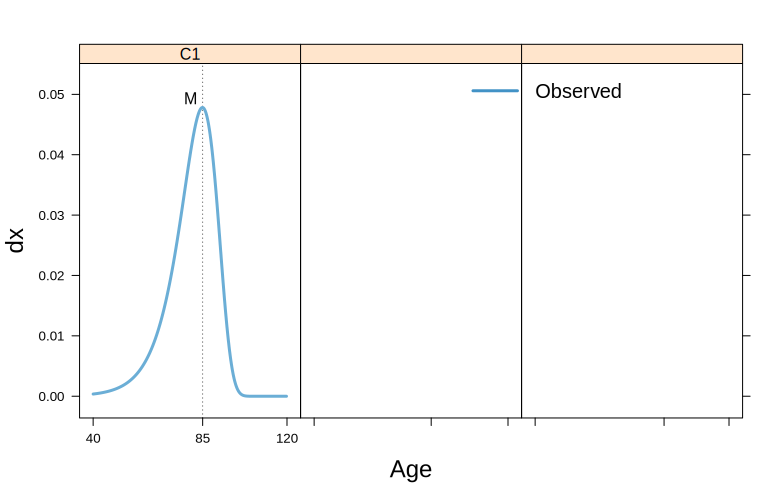
\includegraphics[scale=0.56]{Figures/Ch4/F4_c1_new}
	\end{center}
	
\end{frame}

%%%%%%%%%%%%%%%%%%%%%%%%%%%%%%%%%%%%%%%%%%%%%%%%%%%%%%%%%%%%%%%%%%%%%%%%%
\begin{frame}[noframenumbering]\frametitle{C-STAD: fully observed $d_x$ ($c_1$)}
	
	\vspace{0.4cm}
	\begin{center}
		\includegraphics[scale=0.56]{Figures/Ch4/F5_CSTAD_1_new}
	\end{center}
	
\end{frame}


%%%%%%%%%%%%%%%%%%%%%%%%%%%%%%%%%%%%%%%%%%%%%%%%%%%%%%%%%%%%%%%%%%%%%%%%%
\begin{frame}\frametitle{C-STAD: partially observed $d_x$ ($c_2$)}
	
	\vspace{0.1cm}
	\begin{center}
		\includegraphics[scale=0.56]{Figures/Ch4/F4_c2_new}
	\end{center}
	
\end{frame}

%%%%%%%%%%%%%%%%%%%%%%%%%%%%%%%%%%%%%%%%%%%%%%%%%%%%%%%%%%%%%%%%%%%%%%%%%
\begin{frame}[noframenumbering]\frametitle{C-STAD: partially observed $d_x$ ($c_2$)}
	
	\vspace{0.4cm}
	\begin{center}
		\includegraphics[scale=0.56]{Figures/Ch4/F5_CSTAD_2_new}
	\end{center}
	
\end{frame}

%%%%%%%%%%%%%%%%%%%%%%%%%%%%%%%%%%%%%%%%%%%%%%%%%%%%%%%%%%%%%%%%%%%%%%%%%
\begin{frame}\frametitle{C-STAD: partially observed $d_x$ ($c_3$)}
	
	\vspace{0.1cm}
	\begin{center}
		\includegraphics[scale=0.56]{Figures/Ch4/F4_c3}
	\end{center}
	
\end{frame}

%%%%%%%%%%%%%%%%%%%%%%%%%%%%%%%%%%%%%%%%%%%%%%%%%%%%%%%%%%%%%%%%%%%%%%%%%
\begin{frame}[noframenumbering]\frametitle{C-STAD: partially observed $d_x$ ($c_3$)}
	
	\vspace{0.4cm}
	\begin{center}
		\includegraphics[scale=0.56]{Figures/Ch4/F5_CSTAD_3}
	\end{center}
	
\end{frame}

%%%%%%%%%%%%%%%%%%%%%%%%%%%%%%%%%%%%%%%%%%%%%%%%%%%%%%%%%%%%%%%%%%%%%%%%%
\begin{frame}\frametitle{C-STAD: summary measures}
	
	\vspace{-0.5cm}
%	
%	\hfill{\hyperlink{CSTADrates}{} $\,$ \hyperlink{CSTADdistributions}{}} 
	
	\begin{center}	
		\vspace{0.4cm}
		
		\includegraphics[scale=.41]{Figures/Ch4/F6_1}
		
	\end{center}
		
\vspace{-0.15cm}
\tiny{$\quad\quad$ Swedish and Danish females, ages 40--110+, cohorts 1835--1970.}

\end{frame}

%%%%%%%%%%%%%%%%%%%%%%%%%%%%%%%%%%%%%%%%%%%%%%%%%%%%%%%%%%%%%%%%%%%%%%%%%%
%\begin{frame}[noframenumbering]\frametitle{C-STAD: results}
%	
%	\vspace{-0.5cm}
%	
%	\hfill{\hyperlink{CSTADrates}{} $\,$ \hyperlink{CSTADdistributions}{}} 
%	
%	\begin{center}	
%		\vspace{0.2cm}
%		
%		\includegraphics[scale=.42]{Figures/Ch4/F6_2}
%		
%	\end{center}
%	
%\end{frame}

%%%%%%%%%%%%%%%%%%%%%%%%%%%%%%%%%%%%%%%%%%%%%%%%%%%%%%%%%%%%%%%%%%%%%%%%%
\begin{frame}[noframenumbering]\frametitle{C-STAD: summary measures}
	
\vspace{-0.5cm}

%\hfill{\hyperlink{CSTADrates}{\beamerbutton{rates}} $\,$ \hyperlink{CSTADdistributions}{\beamerbutton{distributions}}} 
%\hypertarget{CSTADratesBACK}{} 
%\hypertarget{CSTADdistributionsBACK}{}

\begin{center}	
	\vspace{0.4cm}
	
	\includegraphics[scale=.41]{Figures/Ch4/F6_3}
	
\end{center}
	
\vspace{-0.15cm}
\tiny{$\quad\quad$ Swedish and Danish females, ages 40--110+, cohorts 1835--1970.}

	
\end{frame}


%%%%%%%%%%%%%%%%%%%%%%%%%%%%%%%%%%%%%%%%%%%%%%%%%%%%%%%%%%%%%%%%%%%%%
%%%%%%%%% CHAPTER 5 %%%%%%%%%%%%%%%%%%%%%%%%%%%%%%%%%%%%%%%%%%%%%%
%%%%%%%%%%%%%%%%%%%%%%%%%%%%%%%%%%%%%%%%%%%%%%%%%%%%%%%%%%%%%%%%%%%%%
\section{Chapter 5}
\subsection{The 3C-sLC model}
\begin{frame}[plain]\frametitle{Thesis overview}
	\textbf{Five chapters}: 
	\begin{itemize}
		\scriptsize	
		\item {\pgfsetfillopacity{0.2} Basellini, Canudas-Romo and Lenart (2019). Location--Scale Models in Demography: A Useful Re-parameterization of Mortality Models. {\it European Journal of Population}, {\bf 35}, 645\,--\,673. 	
			
		\item  Basellini and Camarda (2019). Modelling and forecasting adult age-at-death distributions. {\it Population Studies}, {\bf 73}(1), 119\,--\,138. 
			
		\item  Basellini and Camarda (2020). A Three-component Approach to Model and Forecast Age-at-death Distributions. In Mazzuco, S., and Keilman, N. (eds.), {\it Developments in Demographic Forecasting}, Springer. Forthcoming. 
		
		\item Basellini, Kj{\ae}rgaard and Camarda (2020). An age-at-death distribution approach \\ to forecast cohort mortality. {\it Insurance: Mathematics and Economics}, {\bf 91}, 129\,--\,143. }	
		
		\item {\pgfsetfillopacity{1}  Camarda and Basellini. Smoothing, decomposing and forecasting mortality rates. Manuscript under review. }	
	\end{itemize}
	\bigskip
	{\pgfsetfillopacity{1} 
		\textbf{Main goal of PhD thesis}: 
		\begin{itemize}
			\item introduce innovative methods to provide novel insights into the analysis and forecasting of human mortality	
		\end{itemize}
	}
\end{frame}


%%%%%%%% Motivation C-STAD PAPER
\begin{frame} %\frametitle{Introduction}
	\textbf{Background:}
	\begin{itemize}
		\setlength\itemsep{0.5em}
		\item the Lee-Carter (LC) model is the reference and most common forecasting methodology in use 
		\item the model has some limitations that hinder its performance 
	\end{itemize}
	\bigskip \pause
	\textbf{Objective:} overcome the LC shortcomings by taking into account the shape of the mortality age-pattern
	\\ \bigskip \pause
	\textbf{Contribution:} propose the Three-Component smooth Lee-Carter (3C-sLC) model to analyze and forecast mortality
	\begin{itemize}
		\setlength\itemsep{0.5em}
		\item more realistic outcomes, i.e.~smooth age-profiles and wider prediction intervals 
		\item enhanced flexibility and goodness-of-fit thanks to mortality decomposition
	\end{itemize}
	
\end{frame}

%%%%%%%%%%%%%%%%%%%%%%%%%%%%%%%%%%%%%%%%%%%%%%%%%%%%%%%%%%%%%%%%%%%%%%%%%%
%%% LC model - advantages/disadvantages
%\begin{frame}          
%	\frametitle{Motivation: the Lee-Carter model (1992)}
%	
%	\textbf{Advantages}:
%	\begin{itemize}
%		\setlength\itemsep{0.5em}	
%		\item simple log-bilinear model: $\ln (m_{x,t}) = \alpha_x + \beta_x\kappa_t + \epsilon_{x,t}$ 
%		\item forecasting is easy: RW model with drift for $\kappa_t$ 
%		\item stochasticity: probabilistic intervals, no ``expert" opinion 
%	\end{itemize}
%	\bigskip \pause
%		\textbf{Disadvantages}:
%		\begin{itemize}
%			\setlength\itemsep{0.5em}		
%			\item Normality assumption (from SVD) 
%%			\item probability bands are too narrow
%			\item fixed age-pattern of mortality decline
%			\begin{itemize}
%				\item jaggedness of fitted/forecast age profile
%				\item changing patterns of mortality improvements
%			\end{itemize} 	  
%		\end{itemize}
%	\bigskip \pause
%	\textbf{Goal}: overcome the disadvantages by decomposing the mortality age-pattern as in the 3C-STAD model (Chapter 3)	
%	
%\end{frame}

%%%%%%%%%%%%%%%%%%%%%%%%%%%%%%%%%%%%%%%%%%%%%%%%%%%%%%%%%%%%%%%%%%%%%%%%%
%% ALPHAS 
\begin{frame}          
	\frametitle{Shape of mortality pattern}
%	\vspace{-0.5cm}
	\begin{center}
%		\vspace{0.2cm}
		\includegraphics[scale=0.41]{Figures/Ch5/Alpha1}
	\end{center}

\vspace{-0.35cm}
\tiny{$\quad\quad$ Log-mortality rates and $\bm{\hat{\alpha}}$ estimates from the LC and 3C-sLC model. \\ $\quad\quad$ Swedish and Danish males, ages 0--100, years 1960--2016.}

	
\end{frame}

%%%%%%%%%%%%%%%%%%%%%%%%%%%%%%%%%%%%%%%%%%%%%%%%%%%%%%%%%%%%%%%%%%%%%%%%%
%%  ALPHAS 
\begin{frame}[noframenumbering]           
	\frametitle{Shape of mortality pattern}
%	\vspace{-0.5cm}
	\begin{center}
%		\vspace{0.2cm}
		\includegraphics[scale=0.41]{Figures/Ch5/Alpha2}
	\end{center}

\vspace{-0.35cm}
\tiny{$\quad\quad$  Log-mortality rates and $\bm{\hat{\alpha}}$ estimates from the LC and 3C-sLC model. \\ $\quad\quad$ Swedish and Danish males, ages 0--100, years 1960--2016.}
	
\end{frame}

%%%%%%%%%%%%%%%%%%%%%%%%%%%%%%%%%%%%%%%%%%%%%%%%%%%%%%%%%%%%%%%%%%%%%%%%%
%%  ALPHAS 
\begin{frame}[noframenumbering]           
	\frametitle{Shape of mortality pattern}
%	\vspace{-0.5cm}
	\begin{center}
%		\vspace{0.2cm}
		\includegraphics[scale=0.41]{Figures/Ch5/Alpha3}
	\end{center}

\vspace{-0.35cm}
\tiny{$\quad\quad$ Log-mortality rates and $\bm{\hat{\alpha}}$ estimates from the LC and 3C-sLC model. \\ $\quad\quad$ Swedish and Danish males, ages 0--100, years 1960--2016.}
	
\end{frame}

%%%%%%%%%%%%%%%%%%%%%%%%%%%%%%%%%%%%%%%%%%%%%%%%%%%%%%%%%%%%%%%%%%%%%%%%%
%% BETAS 
\begin{frame}          
	\frametitle{Rates of mortality improvement}
	%	\vspace{-0.5cm}
	\begin{center}
		%		\vspace{0.2cm}
		\includegraphics[scale=0.41]{Figures/Ch5/Beta1}
	\end{center}
	
	\vspace{-0.35cm}
\tiny{$\quad\quad$ $\bm{\hat{\beta}}$ estimates from the LC and 3C-sLC model. \\ $\quad\quad$ Swedish and Danish males, ages 0--100, years 1960--2016.}
\end{frame}

%%%%%%%%%%%%%%%%%%%%%%%%%%%%%%%%%%%%%%%%%%%%%%%%%%%%%%%%%%%%%%%%%%%%%%%%%
%%  BETAS 
\begin{frame}[noframenumbering]           
	\frametitle{Rates of mortality improvement}
	%	\vspace{-0.5cm}
	\begin{center}
		%		\vspace{0.2cm}
		\includegraphics[scale=0.41]{Figures/Ch5/Beta2}
	\end{center}
		\vspace{-0.35cm}
\tiny{$\quad\quad$ $\bm{\hat{\beta}}$ estimates from the LC and 3C-sLC model. \\ $\quad\quad$ Swedish and Danish males, ages 0--100, years 1960--2016.}

\end{frame}

%%%%%%%%%%%%%%%%%%%%%%%%%%%%%%%%%%%%%%%%%%%%%%%%%%%%%%%%%%%%%%%%%%%%%%%%%
%%  KAPPAS
\begin{frame}           
	\frametitle{Level of mortality}
	
	\vspace{-0.25cm}
	
	\begin{center}
		\includegraphics[scale=0.41]{Figures/Ch5/KappaFore1_M}
	\end{center}
\vspace{-0.3cm}	
\tiny{$\quad\quad$ $\bm{\hat{\kappa}}$ estimates and forecasts from the LC and 3C-sLC model. \\ $\quad\quad$ Swedish and Danish males, ages 0--100, fitted years 1960--2016, forecast years 2017--2040.}
	
\end{frame}

%%%%%%%%%%%%%%%%%%%%%%%%%%%%%%%%%%%%%%%%%%%%%%%%%%%%%%%%%%%%%%%%%%%%%%%%%
%%  3CsLC FORECASTING KAPPAS
\begin{frame}[noframenumbering]           
	\frametitle{Level of mortality}
	
	\vspace{-0.25cm}
	
	\begin{center}
		\includegraphics[scale=0.41]{Figures/Ch5/KappaFore2_M}
	\end{center}

\vspace{-0.3cm}	
\tiny{$\quad\quad$ $\bm{\hat{\kappa}}$ estimates and forecasts from the LC and 3C-sLC model. \\ $\quad\quad$ Swedish and Danish males, ages 0--100, fitted years 1960--2016, forecast years 2017--2040.}
	
\end{frame}

%%%%%%%%%%%%%%%%%%%%%%%%%%%%%%%%%%%%%%%%%%%%%%%%%%%%%%%%%%%%%%%%%%%%%%%%%
%%  3CsLC FORECASTING KAPPAS
\begin{frame}[noframenumbering]           
	\frametitle{Level of mortality}
	
	\vspace{-0.25cm}
	
	\begin{center}
		\includegraphics[scale=0.41]{Figures/Ch5/KappaFore3_M}
	\end{center}

\vspace{-0.3cm}	
\tiny{$\quad\quad$ $\bm{\hat{\kappa}}$ estimates and forecasts from the LC and 3C-sLC model. \\ $\quad\quad$ Swedish and Danish males, ages 0--100, fitted years 1960--2016, forecast years 2017--2040.}
	
\end{frame}

%%%%%%%%%%%%%%%%%%%%%%%%%%%%%%%%%%%%%%%%%%%%%%%%%%%%%%%%%%%%%%%%%%%%%%%%%%
%%% KAPPAS 
%\begin{frame}          
%	\frametitle{The 3C-sLC model: $\kappa_i$}
%	%	\vspace{-0.5cm}
%	\begin{center}
%		%		\vspace{0.2cm}
%		\includegraphics[scale=0.42]{Figures/Ch5/Kappa1}
%	\end{center}
%	
%\end{frame}
%
%%%%%%%%%%%%%%%%%%%%%%%%%%%%%%%%%%%%%%%%%%%%%%%%%%%%%%%%%%%%%%%%%%%%%%%%%%
%%%  KAPPAS 
%\begin{frame}[noframenumbering]           
%	\frametitle{The 3C-sLC model: $\kappa_i$}
%	%	\vspace{-0.5cm}
%	\begin{center}
%		%		\vspace{0.2cm}
%		\includegraphics[scale=0.42]{Figures/Ch5/Kappa2}
%	\end{center}
%	
%\end{frame}


%%%%%%%%%%%%%%%%%%%%%%%%%%%%%%%%%%%%%%%%%%%%%%%%%%%%%%%%%%%%%%%%%%%%%%%%%
%%  3CsLC component FITTING 
\begin{frame}           
	\frametitle{3C-sLC: components}
	
	\vspace{-0.35cm}
	
	\begin{center}
%		\animategraphics[autoplay,scale=0.425]{3}{Figures/Ch5/RATES3CsLC}{0}{21}
	\includegraphics[scale=.42]{Figures/Ch5/RATES_FIT_M}
	
	\end{center}

\vspace{-0.2cm}	
\tiny{$\quad\quad$ Fitted and forecast components (log-scale) of the 3C-sLC model. \\ $\quad\quad$ Swedish and Danish males, ages 0--100, fitted years 1960--2016, forecast years 2017--2040.}
	
\end{frame}

%%%%%%%%%%%%%%%%%%%%%%%%%%%%%%%%%%%%%%%%%%%%%%%%%%%%%%%%%%%%%%%%%%%%%%%%%
%%  3CsLC component FORECAST 
\begin{frame}           
	\frametitle{3C-sLC: components}
	
	\vspace{-0.35cm}
	
	\begin{center}
%		\animategraphics[autoplay,scale=0.425]{3}{Figures/Ch5/RATES3CsLC}{0}{21}
	\includegraphics[scale=.42]{Figures/Ch5/RATES_FORE_M}
	
	\end{center}
	
\vspace{-0.2cm}	
\tiny{$\quad\quad$ Fitted and forecast components (log-scale) of the 3C-sLC model. \\ $\quad\quad$ Swedish and Danish males, ages 0--100, fitted years 1960--2016, forecast years 2017--2040.}	
\end{frame}

%%%%%%%%%%%%%%%%%%%%%%%%%%%%%%%%%%%%%%%%%%%%%%%%%%%%%%%%%%%%%%%%%%%%%%%%%%
%%%  3CsLC FORECASTING KAPPAS
%\begin{frame}           
%	\frametitle{Forecasting time indices}
%	
%	%	\vspace{0.2cm}
%	
%	\begin{center}
%		\includegraphics[scale=0.425]{Figures/Ch5/KappaFore1}
%	\end{center}
%	
%\end{frame}
%
%%%%%%%%%%%%%%%%%%%%%%%%%%%%%%%%%%%%%%%%%%%%%%%%%%%%%%%%%%%%%%%%%%%%%%%%%%
%%%  3CsLC FORECASTING KAPPAS
%\begin{frame}[noframenumbering]           
%	\frametitle{Forecasting time indices}
%	
%	%	\vspace{0.2cm}
%	
%	\begin{center}
%		\includegraphics[scale=0.425]{Figures/Ch5/KappaFore2}
%	\end{center}
%	
%\end{frame}

%%%%%%%%%%%%%%%%%%%%%%%%%%%%%%%%%%%%%%%%%%%%%%%%%%%%%%%%%%%%%%%%%%%%%%%%%%
%%%  3CsLC component FORECASTING 
%\begin{frame}           
%	\frametitle{Forecasting: components}
%	
%	%	\vspace{0.2cm}
%	
%	\begin{center}
%		\animategraphics[autoplay,scale=0.425]{3}{Figures/Ch5/RATES3CsLC_FORE}{0}{11}
%	\end{center}
%	
%\end{frame}

%%%% RESULTS: FORECASTS 3C-sLC vs LC
\begin{frame}\frametitle{3C-sLC: summary measures}

\vspace{-0.5cm}
	
	\begin{center}	
		\vspace{0.4cm}
		
		\includegraphics[scale=.42]{Figures/Ch5/F1_1_M}
		
	\end{center}

\vspace{-0.3cm}
\tiny{$\quad\quad$ Swedish and Danish males. \\ $\quad\quad$ Ages 0--110+, fitted years 1960--2016, forecast years 2017--2040.}
	
\end{frame}

%%%% RESULTS: FORECASTS 3C-sLC vs LC
\begin{frame}[noframenumbering]\frametitle{3C-sLC: summary measures}

\vspace{-0.5cm}
	
	\begin{center}	
		\vspace{0.4cm}
		
		\includegraphics[scale=.42]{Figures/Ch5/F1_2_M}
		
	\end{center}

\vspace{-0.3cm}
\tiny{$\quad\quad$ Swedish and Danish males. \\ $\quad\quad$ Ages 0--110+, fitted years 1960--2016, forecast years 2017--2040.}
	
\end{frame}

%%%% RESULTS: FORECASTS 3C-sLC vs LC
\begin{frame}[noframenumbering]\frametitle{3C-sLC: summary measures}

\vspace{-0.5cm}
	
	\begin{center}	
		\vspace{0.4cm}
		
		\includegraphics[scale=.42]{Figures/Ch5/F1_3_M}
		
	\end{center}

\vspace{-0.3cm}
\tiny{$\quad\quad$ Swedish and Danish males. \\ $\quad\quad$ Ages 0--110+, fitted years 1960--2016, forecast years 2017--2040.}
	
\end{frame}

%%%%%%%%%%%%%%%%%%%%%%%%%%%%%%%%%%%%%%%%%%%%%%%%%%%%%%%%%%%%%%%%%%%%%
%%%%%%%%% CONCLUSION %%%%%%%%%%%%%%%%%%%%%%%%%%%%%%%%%%%%%%%%%%%%%%%%
%%%%%%%%%%%%%%%%%%%%%%%%%%%%%%%%%%%%%%%%%%%%%%%%%%%%%%%%%%%%%%%%%%%%%
\section{Summary}

%% New frame
\begin{frame}[label=summary]\frametitle{Thesis summary}
	\begin{itemize}
		\setlength\itemsep{1.2em}
		\item[] {\usebeamercolor[fg]{structure}Ch.~1}: introduced the location-scale family as a flexible tool for modelling adult mortality and studying mortality dynamics \pause
		\item[] {\usebeamercolor[fg]{structure}Ch.~2, 3, 4}: developed a novel paradigm in mortality forecasting based on age-at-death distributions 
%		\begin{itemize}
%		\item more optimistic forecasts than rate-based models (e.g. Lee-Carter and variants)
%		\item high point and interval forecast accuracy (out-of-sample validation), often superior to other models 
%		\end{itemize}
		\pause
		\item[] {\usebeamercolor[fg]{structure}Ch.~3, 4, 5}: investigated two rather unexplored dimensions in mortality forecasting
		\begin{itemize}
		\item cohort mortality forecasts
		\item decomposition of the mortality age-pattern into childhood, adulthood and senescent components
		\end{itemize}
	\end{itemize}
\end{frame}

%%%%%%%%%%%%%%%%%%%%%%%%%%%%%%%%%%%%%%%%%%%%%%%%%%%%%%%%%%%%%%%%%%%%%%%%
\begin{frame}[noframenumbering]\frametitle{References}
	\scriptsize

\begin{itemize}
\setlength\itemsep{1.2em}	
%	\item[] Basellini and Camarda (2019). Modelling and forecasting adult age-at-death distributions. {\it Population Studies}, {\bf 73}(1), 119\,--\,138.
%	
%	\item[] Basellini, Canudas-Romo and Lenart (2019). Location--Scale Models in Demography: A Useful Re-parameterization of Mortality Models. {\it European Journal of Population}, {\bf 35}, 645\,--\,673.
%	
%	\item[] Basellini, Kj{\ae}rgaard and Camarda (2020). An age-at-death distribution approach \\ to forecast cohort mortality. {\it Insurance: Mathematics and Economics}, {\bf 91}, 129\,--\,143.
	
	\item[] Camarda, Eilers and Gampe (2016). Sums of smooth exponentials to decompose complex series of counts. {\it Statistical Modelling}, {\bf 16}(4), 279\,--\,296.
	
	\item[] Currie, Durban and Eilers (2004). Smoothing and forecasting mortality rates. {\it Statistical Modelling}, {\bf 4}(4), 279\,--\,298.
	
	\item[] Currie (2016). On fitting generalized linear and non-linear models of mortality. {\it Scandinavian Actuarial Journal}, {\bf 4}, 356\,--\,383.
	
	\item[] Eilers and Marx (1996). Flexible smoothing with $B$-splines and penalties (with discussion). {\it Statistical Science}, {\bf 11}(2), 89\,--\,102.
	
	\item[] Forfar, McCutcheon and Wilkie (1988). On graduation by mathematical formula. {\it Journal of the Institute of Actuaries}, {\bf 115}(1), 1\,--\,149.
	
	\item[] Human Mortality Database (2020). University of California, Berkeley (USA) and Max Planck Institute for Demographic Research (Germany). Available at \url{www.mortality.org} or \url{www.humanmortality.de}.

\end{itemize}

\end{frame}

%%%%%%%%%%%%%%%%%%%%%%%%%%%%%%%%%%%%%%%%%%%%%%%%%%%%%%%%%%%%%%%%%%%%%%%%
\begin{frame}[noframenumbering]\frametitle{References}
	\scriptsize
	
\begin{itemize}
	\setlength\itemsep{1.2em}
	
	\item[] Lee and Carter (1992). Modeling and forecasting US mortality. {\it Journal of the American Statistical Association}, {\bf 87}(419), 659\,--\,671.
	
	\item[] Ouellette and Bourbeau (2011). Changes in the age-at-death distribution in four low mortality countries: A nonparametric approach. {\it Demographic Research}, {\bf 25}, 595\,--\,628.
	
	\item[] Ramsay and Silverman (2005). \textit{Functional Data Analysis}. Second edition. New York: Springer-Verlag.
	
	\item[] Thiele (1871). On a Mathematical Formula to express the Rate of Mortality throughout the whole of Life. {\it Journal of the Institute of Actuaries}, {\bf 16}(5), 313\,--\,329.
	
\end{itemize}
	
\end{frame}


%%%%%%%%%%%%%%%%%%%%%%%%%%%%%%%%%%%%%%%%%%%%%%%%%%%%%%%%%%%%%%%%%%%%%%%%
\begin{frame}[noframenumbering]\frametitle{Acknowledgments}

\small

\begin{itemize}
	\setlength\itemsep{1em}
	
	\item[] Annette Baudisch, Vladimir Canudas-Romo, Jim Oeppen and Giancarlo Camarda \pause
	
	\item[] Marco Bonetti, Tim Crayford and James W.~Vaupel	\pause
	
	\item[] Marie-Pier, Anthony, Marius, Jos{\'e}, Silvia, Marteen, S{\o}ren, Pancho, Jes{\'u}s, Catalina, Ilya and Virginia   \pause
	
	\item[] Alessandro, Matteo, Giulia, Russel, Davide, Sebastian, Namrata, Matthew, Jenny, Enrica, Alessandra, Linh, Enrique, Marcus and Angelo  \pause
	
	\item[]	Mar{\'i}lia, my parents Elena and Aldo, my brother Carlo and Olivia, my grandparents Michela and Gustavo
	
\end{itemize}

\end{frame}

%%%%%%%%%%%%%%%%%%%%%%%%%%%%%%%%%%%%%%%%%%%%%%%%%%%%%%%%%%%%%%%%%%%%%%%%
\begin{frame}\frametitle{$\,$}
	\vspace{-1.5cm}
	\begin{center}
	\begin{Large}	
	{\usebeamercolor[fg]{structure} \textsc{New Approaches in Mortality \\ Modelling and Forecasting} \\}
	\end{Large}
	\bigskip 
		\bigskip 

	\begin{large}
	{\usebeamercolor[fg]{structure} \textit{Assessment of PhD dissertation}} \\
	\bigskip
				\bigskip 
	Ugofilippo Basellini 
	\end{large}	
	\bigskip
	\bigskip
	\bigskip
	
	\begin{large}	
	\textsl{Thank you for your attention!}
	\end{large}	
	\end{center}
	\bigskip
	\bigskip
	\bigskip
	
\end{frame}

\againframe<3>[noframenumbering]{summary}


%%%%%%%%%%%%%%%%%%%%%%%%%%%%%%%%%%%%%%%%%%%%%%%%%%%%%%%%%%%%%%%%%%%%%
%%%%%%%%% APPENDICES %%%%%%%%%%%%%%%%%%%%%%%%%%%%%%%%%%%%%%%%%%%%%%%%
%%%%%%%%%%%%%%%%%%%%%%%%%%%%%%%%%%%%%%%%%%%%%%%%%%%%%%%%%%%%%%%%%%%%%
\section*{Appendix}

%% New frame
\begin{frame}[noframenumbering]\frametitle{Future research}
	\begin{itemize}
		\setlength\itemsep{1.35em}
		\item {\usebeamercolor[fg]{structure}Applicability}:  broader application of methodologies to other populations, e.g.:
		\begin{itemize}
			\item other low-mortality populations
			\item populations with lower data quality
			\item populations with atypical mortality developments 
		\end{itemize}
		\item {\usebeamercolor[fg]{structure}Generalization}: extension of methodologies to other datasets, e.g.~causes-of-death, fertility, coherent mortality projections
		\item
		{\usebeamercolor[fg]{structure}Distribution}: development of an \texttt{R} package for fast(er) implementation and use of the methodologies
	\end{itemize}
\end{frame}

%%%%%%%% ADDITIONAL SLIDES (HYPERTARGETS)

%%%%%%%% SOME SLIDES ON THREE MORTALITY MODELS (FOR PAPER 1)
%%%%%%%% SOME SLIDES ON THREE MORTALITY MODELS (FOR PAPER 1)
%% Frame A
%\begin{frame}[noframenumbering]
%\vspace{0.35cm}
%\begin{center}
%\includegraphics[scale=0.5]{Figures/Ch1/F1_a}
%\end{center}
%\vspace{-0.5cm}
%\scriptsize{\emph{$\quad\quad\quad\quad\;$ Source: HMD (2020)}}
%\hfill{\hyperlink{ParamModelsBACK}{\beamerbutton{go back}}}
%\\
%\hypertarget{ParamModels}{}
%\end{frame}
%
%%% Frame B
%\begin{frame}[noframenumbering]
%\vspace{0.35cm}
%\begin{center}
%\includegraphics[scale=0.5]{Figures/Ch1/F1_b}
%\end{center}
%\vspace{-0.5cm}
%\scriptsize{\emph{$\quad\quad\quad\quad\;$ Source: HMD (2020)}}
%\hfill{\hyperlink{ParamModelsBACK}{\beamerbutton{go back}}}
%\end{frame}
%
%%% Frame C
%\begin{frame}[noframenumbering]
%\vspace{0.35cm}
%\begin{center}
%\includegraphics[scale=0.5]{Figures/Ch1/F1_c}
%\end{center}
%\vspace{-0.5cm}
%\scriptsize{\emph{$\quad\quad\quad\quad\;$ Source: HMD (2020)}}
%\hfill{\hyperlink{ParamModelsBACK}{\beamerbutton{go back}}}
%\end{frame}

%% Frame D
%\begin{frame}[noframenumbering]
%\vspace{0.35cm}
%\begin{center}
%\includegraphics[scale=0.5]{Figures/Ch1/F1_d}
%\end{center}
%\vspace{-0.5cm}
%\scriptsize{\emph{$\quad\quad\quad\quad\;$ Source: HMD (2020)}}
%\hfill{\hyperlink{ParamModelsBACK}{\beamerbutton{go back}}}
%\end{frame}

%%%%%%%% LIST OF LS MORTALITY MODELS 
%%%%%%%% LIST OF LS MORTALITY MODELS 
%% Frame A
\begin{frame}[noframenumbering]
\frametitle{LS mortality models}

\begin{table}[]
\begin{tabular}{@{}l|l|l@{}}
\toprule
\begin{tabular}[c]{@{}l@{}}Models belonging \\ to LS family\end{tabular} & \begin{tabular}[c]{@{}l@{}}Models belonging \\ to LLS family\end{tabular} & \begin{tabular}[c]{@{}l@{}}Models related\\ to LS family\end{tabular}         \\ \midrule
Logistic                                                                 & Log--Logistic                                                            & Gompertz                                                                      \\
\rowcolor{grey}  
Normal                                                                   & Log--Normal                                                            & Kannisto                                                                      \\
\begin{tabular}[c]{@{}l@{}}Smallest \\ Extreme--Value\end{tabular}       & Weibull                                                              & Gamma--Gompertz                     \\
\rowcolor{grey} 
\begin{tabular}[c]{@{}l@{}}Largest\\ Extreme--Value\end{tabular}         &                                                                          & \begin{tabular}[c]{@{}l@{}}Minimal Generalized \\ Extreme--Value\end{tabular} \\
                                                                         &                                                                          & \begin{tabular}[c]{@{}l@{}}Maximal Generalized \\ Extreme--Value\end{tabular} \\ \bottomrule
\end{tabular}
\end{table}

\bigskip

%\hfill{\hyperlink{LSModelsBACK}{\beamerbutton{go back}}}
%\\
%\hypertarget{LSModels}{}
\end{frame}

%% Contribution to changes in e30
\begin{frame}[noframenumbering]
	\frametitle{LS contributions to changes in $e_{30}$}
	\vspace{-0.25cm}
	\begin{center}
		\includegraphics[scale=0.32]{Figures/Ch1/F5a}\includegraphics[scale=0.32]{Figures/Ch1/F5b}
	\end{center}
	\vspace{-0.3cm}
	\tiny{$\quad\quad\quad\quad$ Contributions of the location $u$ (green) and scale $c$ (light blue) Gompertz
parameters to changes in $e_{30}$.\\ $\quad\quad\quad\quad$ Swedish and Danish females, ages 30--110+, years 1960--2015. \\ \emph{$\quad\quad\quad\quad$ Source: Basellini et al. (2019)}} \\
	%\hfill{\hyperlink{LSOtherModelsBACK}{\beamerbutton{go back}}}
	%\\
	%\hypertarget{LSOtherModels}{}
\end{frame}

%%%%%%%% DIFFERENT LS MORTALITY MODELS (FOR PAPER 1)
%%%%%%%% DIFFERENT LS MORTALITY MODELS (FOR PAPER 1)
%% Frame A
\begin{frame}[noframenumbering]
\frametitle{LS estimates}
\vspace{-0.25cm}
\begin{center}
\includegraphics[scale=0.45]{Figures/Ch1/F4_a}
\end{center}
\vspace{-0.3cm}
\tiny{$\quad\quad\quad\quad$ Rescaled LS estimated parameters of the Minimal Generalized Extreme--Value model.\\ $\quad\quad\quad\quad$ Danish females, ages 30--110+, years 1960--2016. \\ \emph{$\quad\quad\quad\quad$ Source: HMD (2020)}} \\
%\hfill{\hyperlink{LSOtherModelsBACK}{\beamerbutton{go back}}}
%\\
%\hypertarget{LSOtherModels}{}
\end{frame}

%% Frame B
\begin{frame}[noframenumbering]
\frametitle{LS estimates}
\vspace{-0.25cm}
\begin{center}
\includegraphics[scale=0.45]{Figures/Ch1/F4_b}
\end{center}
\vspace{-0.3cm}
\tiny{$\quad\quad\quad\quad$ Rescaled LS estimated parameters of six LS models.\\ $\quad\quad\quad\quad$ Danish females, ages 30--110+, years 1960--2016. \\ \emph{$\quad\quad\quad\quad$ Source: HMD (2020)}} %\\
%\hfill{\hyperlink{LSOtherModelsBACK}{\beamerbutton{go back}}}
%\\

\end{frame}

%%%%%%%% OTHER LS ADVANTAGES (FOR PAPER 1)
%%%%%%%% OTHER LS ADVANTAGES (FOR PAPER 1)
%% Frame A
\begin{frame}[noframenumbering]
\frametitle{LS correlations}
\vspace{-0.05cm}
\begin{center}
\includegraphics[scale=0.44]{Figures/Ch1/F6}
\end{center}
\vspace{-0.05cm}
\tiny{$\quad\quad\quad\quad$ MLEs and $R^2$ for the classic parameterization of three mortality models.\\ $\quad\quad\quad\quad$ 33 countries by gender, ages 30--110+, years 1960--2016. \\ \emph{$\quad\quad\quad\quad$ Source: HMD (2018), Basellini et al.~(2019)}} 
%\hfill{\hyperlink{LSAdvantagesBACK}{\beamerbutton{go back}}}
%\\
%\hypertarget{LSAdvantages}{}
\end{frame}

%% Frame B
\begin{frame}[noframenumbering]
\frametitle{LS correlations}
\vspace{-0.05cm}
\begin{center}
\includegraphics[scale=0.44]{Figures/Ch1/F7}
\end{center}
\vspace{-0.05cm}
\tiny{$\quad\quad\quad\quad$ MLEs and $R^2$ for the LS parameterization of three mortality models.\\ $\quad\quad\quad\quad$ 33 countries by gender, ages 30--110+, years 1960--2016. \\ \emph{$\quad\quad\quad\quad$ Source: HMD (2018), Basellini et al.~(2019)}} 
%\hfill{\hyperlink{LSAdvantagesBACK}{\beamerbutton{go back}}}
\end{frame}

%% Frame C
\begin{frame}[noframenumbering]
\frametitle{LS correlations}
\vspace{-0.05cm}
\begin{center}
\includegraphics[scale=0.41]{Figures/Ch1/F8}
\end{center}
\vspace{-0.05cm}
\tiny{$\quad\quad\quad\quad$ Within-country absolute correlation of the classic and LS parameterization of three mortality models.\\ $\quad\quad\quad\quad$ 33 countries by gender, ages 30--110+, years 1960--2016. \\ \emph{$\quad\quad\quad\quad$ Source: HMD (2018), Basellini et al.~(2019)}} \\
%\hfill{\hyperlink{LSAdvantagesBACK}{\beamerbutton{go back}}}
\end{frame}

%% Frame B
%\begin{frame}[noframenumbering]
%\frametitle{Results: LS estimates' correlation}
%\vspace{-0.25cm}
%\begin{center}
%\includegraphics[scale=0.45]{Figures/Ch1/F4_b}
%\end{center}
%\vspace{-0.3cm}
%\tiny{$\quad\quad\quad\quad$ Rescaled LS estimated parameters of six LS models.\\ $\quad\quad\quad\quad$ Danish females, ages 30--110+, years 1960--2016. \\ \emph{$\quad\quad\quad\quad$ Source: HMD (2020)}} \\
%\hfill{\hyperlink{LSOtherModelsBACK}{\beamerbutton{go back}}}
%\\
%\end{frame}


%%%%%%%% SOME SLIDES ON PAPER 2
%%%%%%%% SOME SLIDES ON PAPER 2

%%%%%%%%%%%%%%%%%%%%%%%%%%%%%%%%%%%%%%%%%%%%%%%%%%%%%%%%%%%%%%%%%%%%%%%%
\begin{frame}[noframenumbering]\frametitle{STAD: the model}
	
	\textbf{Notation:}
	
	\begin{columns}
		\column{0.47\textwidth}
		\begin{itemize}
			\item $x$: age 
			\item $f(x)$: standard distribution			
		\end{itemize}
		\column{0.53\textwidth}
		\begin{itemize}
			\item $g(x)$: observed distribution	 
			\item $t(x)$: transformation function		
			
		\end{itemize}		
	\end{columns}
	
	\bigskip 
	\bigskip
	
	\textbf{Aim:} Look for a $t(x)$ such that: 
	
	\begin{itemize}
		\item $g(x)$ conforms to $f(x)$ on the warped axis, i.e. $g(x) = f(t(x))$ 
		
		\item $t(\cdot)$ is a \textbf{segmented function} of the difference in modal ages and the change in the variability before and after $M$:
		
		
		\vspace{-0.4cm}
		
		\begin{equation*}\label{eqtx}
			t(x;{\color{Red}s},{\color{Green} b_{L}},{\color{Blue}
				b_{U}}) = \left\{ 
			\begin{array}{ll}
				M^{f} + {\color{Green} b_{L}}\, (x - {\color{Red}s} - M^{f}) \;\;\; & \mathrm{if} \; \; x \leq M^{g} \\
				M^{f} + {\color{Blue} b_{U}}\, (x - {\color{Red}s} - M^{f})  \;\;\; & \mathrm{if} \; \, x >  M^{g} \\
			\end{array}
			\right.
		\end{equation*}	
		
	\end{itemize}
	
\end{frame}

%%%%%%%%%%%%%%%%%%%%%%%%%%%%%%%%%%%%%%%%%%%%%%%%%%%%%%%%%%%%%%%%%%%%%%%%%
\begin{frame}[noframenumbering]\frametitle{STAD: standard distribution}

\vspace{-0.3cm}
	
	\begin{center}
		
		\color{white} \textbf{Landmark registration}: alignment of observed densities to a common mode
		
		\vspace{0.3cm}
		
		\includegraphics[scale=.35]{Figures/Ch2/F8_1.pdf}
		
	\end{center}

\vspace{-0.15cm}
\scriptsize{$\quad\quad\quad\quad$ Source: Basellini et al.~(2019)}
%\hfill{\hyperlink{StandardSTADBACK}{\beamerbutton{go back}}}\\
%\hypertarget{StandardSTAD}{}
	
\end{frame}	

%%%%%%%%%%%%%%%%%%%%%%%%%%%%%%%%%%%%%%%%%%%%%%%%%%%%%%%%%%%%%%%%%%%%%%%%%
\begin{frame}[noframenumbering]\frametitle{STAD: standard distribution}

\vspace{-0.3cm}
	
	\begin{center}
		
		\textbf{Simple mean over ages}: can lead to biased / unreasonable standard distribution 
		
		\vspace{0.3cm}
		
		\includegraphics[scale=.35]{Figures/Ch2/F8_2.pdf}
		
	\end{center}

\vspace{-0.15cm}
\scriptsize{$\quad\quad\quad\quad$ Source: Basellini et al.~(2019)}
%\hfill{\hyperlink{StandardSTADBACK}{\beamerbutton{go back}}}
	
	
\end{frame}	

%%%%%%%%%%%%%%%%%%%%%%%%%%%%%%%%%%%%%%%%%%%%%%%%%%%%%%%%%%%%%%%%%%%%%%%%%
\begin{frame}[noframenumbering]\frametitle{STAD: standard distribution}

\vspace{-0.3cm}
	
	\begin{center}
		
		\textbf{Landmark registration} {\scriptsize (Ramsay \& Silverman 2005)}: alignment of observed densities to a common mode
		
		\vspace{0.3cm}
		
		\includegraphics[scale=.35]{Figures/Ch2/F8_3.pdf}
		
	\end{center}
	
\vspace{-0.15cm}
\scriptsize{$\quad\quad\quad\quad$ Source: Basellini et al.~(2019)}
%\hfill{\hyperlink{StandardSTADBACK}{\beamerbutton{go back}}}

	
\end{frame}	

%%%%%%%%%%%%%%%%%%%%%%%%%%%%%%%%%%%%%%%%%%%%%%%%%%%%%%%%%%%%%%%%%%%%%%%%%
\begin{frame}[noframenumbering]\frametitle{STAD: standard distribution}

\vspace{-0.3cm}
	
	\begin{center}
		
		\textbf{Landmark registration} {\scriptsize (Ramsay \& Silverman 2005)}: alignment of observed densities to a common mode
		
		\vspace{0.3cm}
		
		\includegraphics[scale=.35]{Figures/Ch2/F8_4.pdf}
		
	\end{center}

\vspace{-0.15cm}
\scriptsize{$\quad\quad\quad\quad$ Source: Basellini et al.~(2019)}
%\hfill{\hyperlink{StandardSTADBACK}{\beamerbutton{go back}}}
	
\end{frame}	

%%%% OBSERVED DATA
\begin{frame}[noframenumbering]\frametitle{STAD: application to observed data}
	\vspace{0.4cm}
	\begin{itemize}
		
		%		\item<1-> \textbf{Data:} observed death counts $D_x$ and exposure times $E_x$ for females aged 30+ during 1980-2016 in Sweden and Denmark \scriptsize{(source: HMD 2020)}
		%		\bigskip
		
		\item \textbf{Smoothing} {\scriptsize (Eilers \& Marx 1996)}:
		\begin{itemize}
			\item apply continuous model to discrete data		
			\item avoid rigid parametric mortality structure
			\item derive $M$ and parameter ${\color{Red}s}$ {\scriptsize (Ouellette \& Bourbeau 2011)}
			\item derivation of standard distribution %$\;$ \hyperlink{StandardSTAD}{\beamerbutton{more details}} $\,$ \hypertarget{StandardSTADBACK}{} 
		\end{itemize}
		\bigskip
		
		\item \textbf{Estimation:} for each year, ${\color{Green} b_{L}}$ and ${\color{Blue} b_{U}}$ estimated by maximum likelihood from the assumption: 
		\begin{equation}\label{Eq:Poisson}
		D_{x} \sim \mathcal{P} \, (E_{x} \; \mu_{x}) \notag 
		\end{equation}
	\end{itemize}	
	
	\vspace{0.05cm}
	\begin{center}
		{\scriptsize where $\mu_{x}$ is evaluated numerically from the STAD segmented distribution $f(t(x))$}
		
	\end{center}		
		
\end{frame}

%%%% RESULTS: PARAMETER CORR
\begin{frame}[noframenumbering]\frametitle{STAD: correlations}

\vspace{-0.5cm}
	
%\hfill{\hyperlink{CISTADBACK}{\beamerbutton{go back}}}
%\hypertarget{CISTAD}{} 
	
	\begin{center}	
		\vspace{0.2cm}
		
		\includegraphics[scale=.42]{Figures/Ch2/F_CORR_B}
		
	\end{center}
	
\end{frame}

%%%% RESULTS: PARAMETER CORR
\begin{frame}[noframenumbering]\frametitle{STAD: correlations}

\vspace{-0.5cm}
	
%\hfill{\hyperlink{CISTADBACK}{\beamerbutton{go back}}}
%\hypertarget{CISTAD}{} 
	
	\begin{center}	
		\vspace{0.2cm}
		
		\includegraphics[scale=.42]{Figures/Ch2/F_CORR_S}
		
	\end{center}
	
\end{frame}

%%%% RESULTS: PARAMETER CORR
\begin{frame}[noframenumbering]\frametitle{STAD: correlations}

\vspace{-0.5cm}
 
	
	\begin{center}	
		\vspace{0.2cm}
		
		\includegraphics[scale=.42]{Figures/Ch2/F_CORR_S-BL}
		
	\end{center}
	
\end{frame}

%%%% RESULTS: Summary measures
\begin{frame}[noframenumbering]\frametitle{STAD: overdispersion}

\vspace{-0.5cm}
	
%\hfill{\hyperlink{CISTAD}{} $\,$ \hyperlink{STADrates}{} $\,$ \hyperlink{STADdistributions}{}} 
	
	\begin{center}	
		\vspace{0.4cm}
		
		\includegraphics[scale=.42]{Figures/Ch2/OVERDISP2}
		
	\end{center}

\vspace{-0.3cm}
\tiny{$\quad\quad$ Swedish and Danish females. \\ $\quad\quad$ Ages 30--110+, fitted years 1960--2016, forecast years 2017--2040.}

	
\end{frame}

%%%% RESULTS: SUMMARY MEASURES CI
\begin{frame}[noframenumbering]\frametitle{STAD: CI}

\vspace{-0.5cm}
	
%\hfill{\hyperlink{CISTADBACK}{\beamerbutton{go back}}}
%\hypertarget{CISTAD}{} 
	
	\begin{center}	
		\vspace{0.2cm}
		
		\includegraphics[scale=.42]{Figures/Ch2/F5_1}
		
	\end{center}
	
\end{frame}

%%%% RESULTS: SUMMARY MEASURES CI
\begin{frame}[noframenumbering]\frametitle{STAD: CI}

\vspace{-0.5cm}
	
%\hfill{\hyperlink{CISTADBACK}{\beamerbutton{go back}}}
%\hypertarget{CISTAD}{} 
	
	\begin{center}	
		\vspace{0.2cm}
		
		\includegraphics[scale=.42]{Figures/Ch2/F5_2}
		
	\end{center}
	
\end{frame}

%%%% RESULTS: RATES
\begin{frame}[noframenumbering]\frametitle{STAD: rates}

\vspace{-0.5cm}
%	
%\hfill{\hyperlink{STADratesBACK}{\beamerbutton{go back}}}
%\hypertarget{STADrates}{} 
	
	\begin{center}	
		\vspace{0.2cm}
		
		\includegraphics[scale=.42]{Figures/Ch2/F6_2}
		
	\end{center}
	
\end{frame}

%%%% RESULTS: AAD
\begin{frame}[noframenumbering]\frametitle{STAD: distributions}

\vspace{-0.5cm}
	
%\hfill{\hyperlink{STADdistributionsBACK}{\beamerbutton{go back}}}
%\hypertarget{STADdistributions}{} 
	
	\begin{center}	
		\vspace{0.2cm}
		
		\includegraphics[scale=.42]{Figures/Ch2/F7}
		
	\end{center}
	
\end{frame}


%%%%%%%% SOME SLIDES ON PAPER 3
%%%%%%%% SOME SLIDES ON PAPER 3

%%%% RESULTS: PARAMETER CORR
\begin{frame}[noframenumbering]\frametitle{3C-STAD: correlations}

\vspace{-0.5cm}
	
	
	\begin{center}	
		\vspace{0.2cm}
		
		\includegraphics[scale=.42]{Figures/Ch3/F_CORR_EA}
		
	\end{center}
	
\end{frame}

%%%% RESULTS: SUMMARY MEASURES CI
\begin{frame}[noframenumbering]\frametitle{3C-STAD: CI}

\vspace{-0.5cm}
%	
%\hfill{\hyperlink{CI3CSTADBACK}{\beamerbutton{go back}}}
%\hypertarget{CI3CSTAD}{} 
	
	\begin{center}	
		\vspace{0.2cm}
		
		\includegraphics[scale=.42]{Figures/Ch3/F4_a2}
		
	\end{center}
	
\end{frame}

%%%% RESULTS: SUMMARY MEASURES CI
\begin{frame}[noframenumbering]\frametitle{3C-STAD: CI}

\vspace{-0.5cm}
	
%\hfill{\hyperlink{CI3CSTADBACK}{\beamerbutton{go back}}}
%\hypertarget{CI3CSTAD}{} 
	
	\begin{center}	
		\vspace{0.2cm}
		
		\includegraphics[scale=.42]{Figures/Ch3/F4_a3}
		
	\end{center}
	
\end{frame}


%%%% RESULTS: RATES
\begin{frame}[noframenumbering]\frametitle{3C-STAD: rates}

\vspace{-0.5cm}
	
%\hfill{\hyperlink{3CSTADratesBACK}{\beamerbutton{go back}}}
%\hypertarget{3CSTADrates}{} 
	
	\begin{center}	
		\vspace{0.2cm}
		
		\includegraphics[scale=.42]{Figures/Ch3/F_rates}
		
	\end{center}
	
\end{frame}

%%%% RESULTS: DISTRIBUTIONS
\begin{frame}[noframenumbering]\frametitle{3C-STAD: distributions}

\vspace{-0.5cm}
	
%\hfill{\hyperlink{3CSTADdistributionsBACK}{\beamerbutton{go back}}}
%\hypertarget{3CSTADdistributions}{} 
	
	\begin{center}	
		\vspace{0.2cm}
		
		\includegraphics[scale=.42]{Figures/Ch3/F_dist}
		
	\end{center}
	
\end{frame}

%%%%%%%% SOME SLIDES ON PAPER 4
%%%%%%%% SOME SLIDES ON PAPER 4

%%%% RESULTS: RATES
\begin{frame}[noframenumbering]\frametitle{C-STAD: rates I}
	
	\vspace{-0.5cm}
	
%	\hfill{\hyperlink{CSTADratesBACK}{\beamerbutton{go back}}}
%	\hypertarget{CSTADrates}{} 
	
	\begin{center}	
		\vspace{0.2cm}
		
		\includegraphics[scale=.42]{Figures/Ch4/F7a}
		
	\end{center}
	
\end{frame}

%%%% RESULTS: RATES
\begin{frame}[noframenumbering]\frametitle{C-STAD: rates II}
	
	\vspace{-0.5cm}
	
	%\hfill{\hyperlink{CSTADratesBACK}{\beamerbutton{go back}}} 
	
	\begin{center}	
		\vspace{0.2cm}
		
		\includegraphics[scale=.42]{Figures/Ch4/F7b}
		
	\end{center}
	
\end{frame}

%%%% RESULTS: AAD
\begin{frame}[noframenumbering]\frametitle{C-STAD: distributions}
	
	\vspace{-0.5cm}
	
%	\hfill{\hyperlink{CSTADdistributionsBACK}{\beamerbutton{go back}}}
%	\hypertarget{CSTADdistributions}{} 
	
	\begin{center}	
		\vspace{0.2cm}
		
		\includegraphics[scale=.42]{Figures/Ch4/F8}
		
	\end{center}
	
\end{frame}


\end{document}
